\documentclass[8pt]{extarticle}
\title{}
\author{Avinash Iyer}
\date{}
\usepackage[shortlabels]{enumitem}

%font setup
%
%\usepackage{newpxtext,eulerpx}

%paper setup
\usepackage{geometry}
\geometry{letterpaper, portrait, margin=1in}
\usepackage{fancyhdr}

%symbols
\usepackage{amsmath}
\usepackage{amssymb}
\usepackage{mathtools}
\usepackage{hyperref}
\usepackage{gensymb}

\usepackage[T1]{fontenc}
\usepackage[utf8]{inputenc}

%chemistry stuff
\usepackage[version=4]{mhchem}
\usepackage{chemfig}

%plotting
\usepackage{pgfplots}
\usepackage{tikz}
\tikzset{middleweight/.style={pos = 0.5, fill=white}}
\tikzset{weight/.style={pos = 0.5, fill = white}}
\tikzset{lateweight/.style={pos = 0.75, fill = white}}
\tikzset{earlyweight/.style={pos = 0.25, fill=white}}

%\usepackage{natbib}

%graphics stuff
\usepackage{graphicx}
\usepackage{svg}
\graphicspath{ {./images/} }

%code stuff
%when using minted, make sure to add the -shell-escape flag
%you can use lstlisting if you don't want to use minted
%\usepackage{minted}
%\usemintedstyle{pastie}
%\newminted[javacode]{java}{frame=lines,framesep=2mm,linenos=true,fontsize=\footnotesize,tabsize=3,autogobble,}
%\newminted[cppcode]{cpp}{frame=lines,framesep=2mm,linenos=true,fontsize=\footnotesize,tabsize=3,autogobble,}

\usepackage{listings}
\usepackage{color}
\definecolor{dkgreen}{rgb}{0,0.6,0}
\definecolor{gray}{rgb}{0.5,0.5,0.5}
\definecolor{mauve}{rgb}{0.58,0,0.82}

\lstset{frame=tb,
	language=Java,
	aboveskip=3mm,
	belowskip=3mm,
	showstringspaces=false,
	columns=flexible,
	basicstyle={\small\ttfamily},
	numbers=none,
	numberstyle=\tiny\color{gray},
	keywordstyle=\color{blue},
	commentstyle=\color{dkgreen},
	stringstyle=\color{mauve},
	breaklines=true,
	breakatwhitespace=true,
	tabsize=3
}
% text + color boxes
\usepackage[most]{tcolorbox}
\tcbuselibrary{breakable}
\newtcolorbox{problem}[1]{colback = white, title = {#1}, breakable}
\newtcolorbox{solution}{colback = white, colframe = black!75!white, title = Solution, breakable}
%including PDFs
\usepackage{pdfpages}
\setlength{\parindent}{0pt}

\newcommand{\card}{\text{card}}
\newcommand{\ran}{\text{ran}}
\newcommand{\N}{\mathbb{N}}
\newcommand{\Q}{\mathbb{Q}}
\newcommand{\Z}{\mathbb{Z}}
\newcommand{\R}{\mathbb{R}}
\pagestyle{fancy}
\fancyhf{}
\rhead{Avinash Iyer}
\lhead{Math 212: Class Notes}
\begin{document}
\renewcommand{\arraystretch}{1.5}
  \begin{problem}{The basis of Multivariable Calculus}
    If a function is continuous and differentiable, on a small enough interval, the function will approximate a line (i.e., a function of $x$).\\

    A similar intuition applies to functions of more than one variable (but with a plane, cube, hypercube, etc.). However, in multivariable functions, we will have to sacrifice the ability to visualize it.\\

    For example, in multiple dimensions, it is possible for there to be a function that is both strictly decreasing (in one dimension) and strictly increasing (in another dimension).
  \end{problem}
  \begin{problem}{Some Functions and Sets}
    \[
      f(x,y) = x^2-y^2
    \] 
    \begin{description}[font=\normalfont\scshape]
      \item[Domain:]  $\{(x,y)\mid \exists f(x,y)\}$
      \item[Range:] $\{f(x,y) \mid (x,y)\in \textrm{Dom}(f)\} = \mathbb{R}$
      \item[Graph:] $\textrm{Graph}(f) = \{x,y.f(x,y) \mid x,y\in \textrm{Dom}(f)\}$. For example, $(1,3,4)\notin \textrm{Graph}(f)$ since $1^2-3^2 \neq 4$.
    \end{description}
  \end{problem}
  \begin{problem}{Examples}
    In $\mathbb{R}^3$, in $x,y,z$ coordinates, $z=3$ is a plane defined as follows:
    \begin{itemize}
      \item Parallel to the $xy$ plane.
      \item Passes through the point $(0.0,3)$.
    \end{itemize}
    \begin{center}
      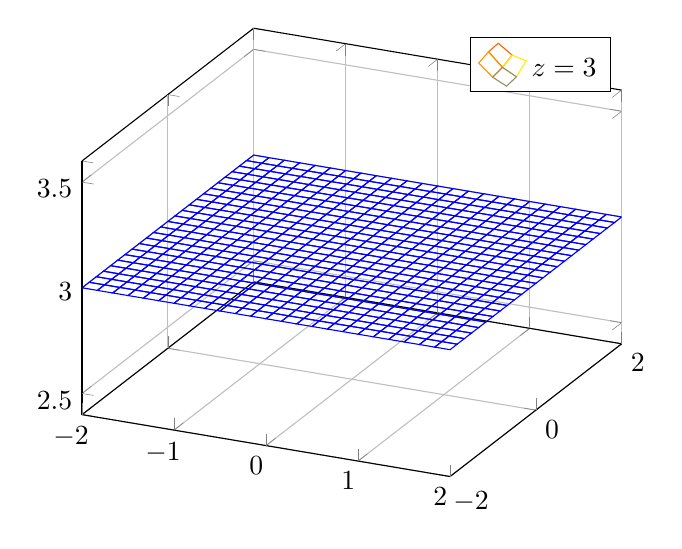
\begin{tikzpicture}
        \begin{axis}[grid=major]
          \addplot3[mesh,domain=-2:2,y domain=-2:2]{3};
          \addlegendentry{$z = 3$}
        \end{axis}
      \end{tikzpicture}
    \end{center}
    Meanwhile, $y=0$ would be a ``wall'' that passes through the origin that contains the line $y=0$ in the $xy$ plane.\\

    Finally, $z = x+y+1$ is a plane, as we can see below.
    \begin{center}
      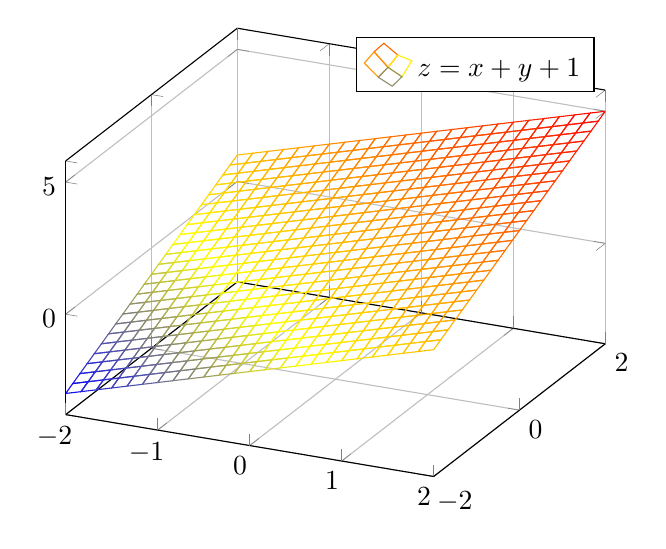
\begin{tikzpicture}
        \begin{axis}[grid=major]
          \addplot3[mesh,domain=-2:2,y domain=-2:2]{x+y+1};
          \addlegendentry{$z = x+y+1$}
        \end{axis}
      \end{tikzpicture}
    \end{center}
  \end{problem}
  \begin{problem}{Visualizing a function of multiple variables}
    Consider the function $f(x,y) = x^2-y^2$. We can try visualizing slices as follows:
    \begin{itemize}
      \item $f(-2,y) = 4-y^2$
      \item $f(0,y) = -y^2$
      \item $f(2,y) = 4-y^2$
      \item $f(x,-2) = x^2+4$
      \item $f(x,0) = x^2$
      \item $f(x,2) = x^2+4$
    \end{itemize}
    %\begin{center}
    %  \begin{tikzpicture}
    %    \begin{axis}[grid=major]
    %      \addplot3[mesh,domain=-4:4,y domain=-4:4]{x^2-y^2};
    %      \addlegendentry{$z = x+y+1$}
    %    \end{axis}
    %  \end{tikzpicture}
    %\end{center}
    Alternatively, we can visualize via contour diagrams (i.e., everywhere that $z$ is a certain value), as seen in mathematica as follows:
    \begin{tcbraster}[raster columns = 1,colframe = black!75!white,colback=white, title=Contour Diagram]
      \tcbincludepdf{images/contour_1.pdf}
    \end{tcbraster}
  \end{problem}
  \begin{problem}{Contour Example}
    Consider the function $f(x,y) = y-3x^2$. We want to find the contours.
    \tcblower
    For any $c$, we have that $c = y-3x^3$, or $y = 3x^3 + c$. Therefore, every contour ``looks like'' $3x^3 + c$ for values of $c$. For example, in the following, we have $c = \{-2,-1,0,1,2\}$ 
   \begin{tcbraster}[raster columns = 1,colframe = black!75!white,colback=white]
     \tcbincludepdf{images/contour_2.pdf}
   \end{tcbraster}
  \end{problem}
  \begin{problem}{Distance}
    In $\mathbb{R}^5$, let $p = (3,1,4,1,5)$, and $q = (1,0,-2,0,2)$. Using the Euclidean metric, we can find the distance between $p$ and $q$ is $d(p,q) = ((3-1)^2 + (1-0)^2 + (4-(-2))^2 + (1-0)^2 + (5-2)^2)^{1/2}= (4+1+36+1+9)^{1/2} = \sqrt{51} = 7.14$. We can also call this the $2$-norm.

    \[
      d(p,q) = \left(\sum_{k=1}^{n} (p_k-q_k)^2\right)^{1/2}
    \] 
  \end{problem}
  \begin{problem}{Derivatives}
    \begin{center}
      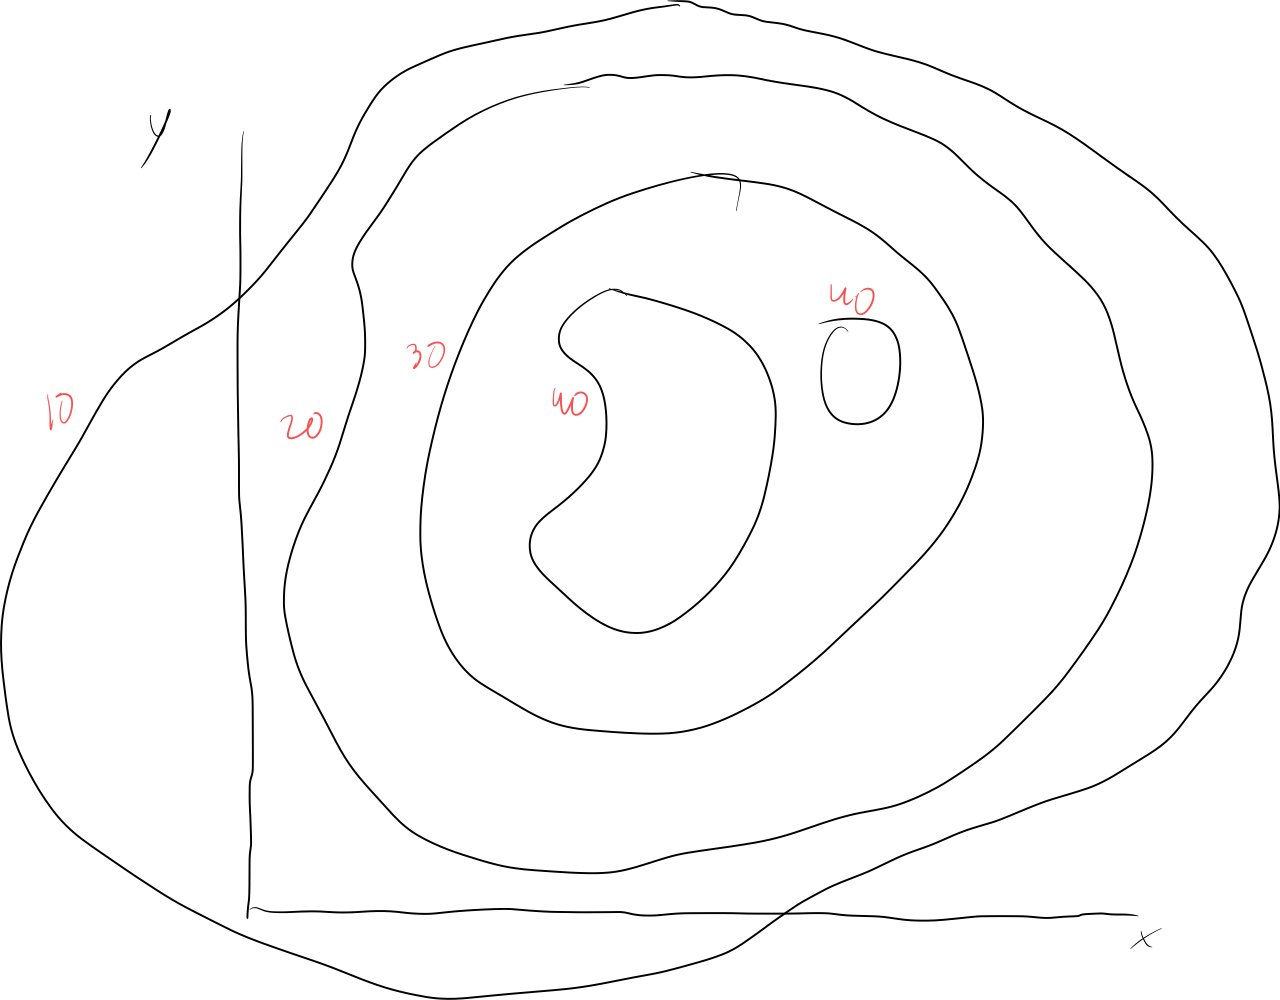
\includegraphics[width=10cm]{contour_3}
    \end{center}
    To denote a derivative, we can't talk about one value, we must use a \textit{partial} derivative, $\frac{\partial f}{\partial x}$, or $\frac{\partial f}{\partial y}$. The closeness of the contours specifies both resolution and steepness.\\

    We can estimate slope by calculating the difference between two contours, divided by the distance between them along a path.\\

    We can also analyze via a table:
    \begin{center}
      \renewcommand{\arraystretch}{1.5}
      \begin{tabular}{c|c|c|c}
        x\symbol{92}y & 0 & 1 & 2 \\
        \cline{2-4}
        4 & 5 & 6 & 7 \\
        \hline
        6 & 8 & 9 & 10 \\
        \hline
        8 & 11 & 12 & 13
      \end{tabular}
    \end{center}
    A ``linear'' approximation for a function of two variables is expressed as follows:
    \[
      z-z_0 = m(x-x_0) + n(y-y_0)
    \] 
    Where $(x_0,y_0,z_0)\in \mathbb{R}^3$, and is an output in $z=f(x,y)$, and $m,n\in \mathbb{R}$.\\

    For example, with the above table, we can see that the function is linear in $x$ and $y$ (i.e., the slope holding the other variable constant is constant).
  \end{problem}
  \begin{problem}{Limits in Multivariable Functions}
    Consider the following:
    \[
      \lim_{(x,y)\rightarrow (0,0)} \frac{x^2 + y^2}{x^2-y^2}
    \] 
    Allow $y = mx$
    \begin{align*}
      \lim_{(x,y)\rightarrow (0,0)} \frac{x^2 + y^2}{x^2-y^2}&= \lim_{(x,y)\rightarrow (0,0)} \frac{x^2 + (mx)^2}{x^2 - (mx)^2}\\
                                                             &= \frac{1+m^2}{1-m^2}
    \end{align*}
    Thus, the limit must depend on the path taken. The following table shows the limits for different values of $m$
    \begin{center}
      \begin{tabular}{c|c}
        $m$ & $\displaystyle\lim_{(x,y)\rightarrow (0,0)} \frac{x^2 + y^2}{x^2 - y^2}$\\
        \hline
        0 & $1$\\
        1 & undefined\\
        2 & $-\frac{5}{3}$
      \end{tabular}
    \end{center}
    Because the limit depends on the path of incidence, we have that the limit is \textbf{undefined}.\\

    For graphs where the contours ``approach'' a particular point, we can see that the limit is defined.
  \end{problem}
  \begin{problem}{Vectors}
    A vector is a mathematical object with direction and magnitude:
    \[
      \vec{v} = \begin{bmatrix}
        3\\1\\4
      \end{bmatrix}
    \] 
    Alternatively, we can have $\vec{w} = \begin{bmatrix}3&1&4\end{bmatrix}$. These vectors are equivalent because they are components of $\mathbb{R}^3$.\\

    Vector addition is \textit{component-wise}, (i.e., you add or subtract components in order to find the new vectors).
    \begin{problem}{Direction of $\vec{v}$}
      \[
        \frac{\vec{v}}{\Vert\vec{v}\Vert}
      \] 
    \end{problem}
    \begin{problem}{Properties of Vectors}
      Let $\vec{u},\vec{v}\in \mathbb{R}^n$. Via properties of the real numbers, we know the following:
      \begin{itemize}
        \item $\vec{u} + \vec{v} = \vec{v} + \vec{u}$
        \item $(\vec{u} + \vec{v}) + \vec{w} = \vec{u} + (\vec{v} + \vec w)$
        \item $c\vec{u} = \langle cu_1,cu_2,\dots,cu_k\rangle$
      \end{itemize}
      Additionally, we define $\vec{u} \cdot \vec{v}$ as follows:
      \[
        \vec{u} \cdot \vec{v} = \sum_{k = 1}^{n} u_kv_k = \Vert\vec{u}\Vert\Vert\vec{v}\Vert\cos\theta
      \] 
    \end{problem}
  \end{problem}
  \begin{problem}{Partial Derivatives}
    Consider $f(x,y) = x^2y + xe^y$.
    \begin{align*}
      f_x &:= \frac{\partial f}{\partial x}\\
      f_x(a,b) &= \frac{\partial f}{\partial x}\biggr\rvert_{(a,b)}
    \end{align*}
    We know that $f\in C^{\infty}(\mathbb{R} \times \mathbb{R})$, meaning $f$ is endlessly differentiable.
  \end{problem}
  \begin{problem}{Functions and Approximations}
    Let $f(x,y) = x^2 - y^2$, $g(x,y) = 2xy$
    \begin{itemize}
      \item $f_{xx} + f_{yy} = 0$
      \item $g_{xx} + g_{yy} = 0$
    \end{itemize}
    This is the solution to the Laplace equation:
    \begin{align*}
      0 &= \frac{\partial^2 f}{\partial x^2} + \frac{\partial^2 f}{\partial y^2}
    \end{align*}
    For $f(x,y)$ at $(a,b,f(a,b))$, we have the following:
    \begin{align*}
      \ell(x,y) &= f(a,b) + f_x(a,b)(x-a) + f_y(y-b)\\
      q(x,y) &= \ell(x,y) + \frac{1}{2}\left(f_{xx}(a,b)(x-a)^2 + 2f_{xy}(a,b)(x-a)(y-b) + f_{yy}(a,b)(y-b)^2\right)\\
    \end{align*}
    In order to get a sense of the ``derivative,'' we can use the following:
    \begin{align*}
      \nabla f(x,y) = \langle f_x(x,y),f_y(x,y)\rangle
    \end{align*}
  \end{problem}
  \begin{problem}{Directional Derivative and Gradient}
    Given $f(x,y)$ and $(a,b)$, where $f\in C^{2}(\mathbb{R}^2)$. Then, the quadratic approximation is:
    \begin{align*}
      f(x,y) &\approx f(a,b) + f_{x}(a,b)(x-a) + f_x(a,b)(y-b)\\
             &+ \frac{1}{2}\left(f_{xx}(a,b)(x-a)^2 + f_{yy}(a,b)(y-b)^2 + f_{xy}(a,b)(x-a)(y-b)\right)\\
          df &= f_x(a,b)dx + f)y(a,b)dy \tag*{a differential}\\
      \Delta f &= f_x(a,b)\Delta x + f_y(a,b)\Delta y\\
      \shortintertext{Evaluating $f(x,y) = xe^y$ at $(a,b) = (-1,0)$}
      f_x &= e^y\\
      f_y &= xe^y\\
      f_x(-1,0) &= 1\\
      f_y(-1,0) &= -1\\
      \Delta f &= \Delta x - \Delta u
    \end{align*}
    On a given contour map, let $\vec u = \langle u_1,u_2\rangle$ denote a \textit{unit} vector in a direction that we want to find the derivative of $f$ in.
    \begin{align*}
      f_{\vec u}(x,y) &= \nabla f(a,b) \cdot \vec u\\
      \shortintertext{Where}
      \nabla f(a,b) &= \langle f_x(a,b),f_y(a,b)\rangle
    \end{align*}
    The directional derivative for all vectors $\vec v$ is as follows:
    \begin{align*}
      f_{\vec v} &= \nabla f \cdot \frac{\vec v}{\Vert \vec v \Vert}
    \end{align*}
  \end{problem}
  \begin{problem}{Chain Rule}
    Let $f(x,y)$ be a function where $x - x(t)$ and $y = y(t)$. We want to find
    \begin{align*}
      \frac{d}{dt}f(x(t),y(t)) &= \frac{\partial f}{\partial x}\frac{dx}{dt} + \frac{\partial f}{\partial y}\frac{dy}{dt}
    \end{align*}
    The chain rule works in higher dimensions too. Consider $k(x_1(t),x_2(t),\dots,x_{152}(t))$. Then,
    \begin{align*}
      \frac{dk}{dt} &= \sum_{i=1}^{152}\frac{\partial k}{\partial x_i}\frac{dx_i}{dt}
    \end{align*}
    We can also view this as a vector. Let $\vec x = \begin{pmatrix}x_{\small 1}(t)\\x_{\small 2}(t)\\\vdots\\x_{\small152}(t)\end{pmatrix}$. Then, we can write $\frac{dk}{dt}$ more succinctly as follows:
    \begin{align*}
      \frac{dk}{dt} = \nabla k \cdot \frac{d\vec x}{dt}
    \end{align*}
    For example, let $f(x,y,z) = 3x^2y + zx + 2$, where $x = x(t),y=y(t),z=z(t)$
    \begin{align*}
      \frac{df}{dt} &= \begin{pmatrix}6xy+z\\3x^2\\x\end{pmatrix} \cdot \begin{pmatrix}x'(t)\\y'(t)\\z'(t)\end{pmatrix}\\
                    &= \left(6xy + z\right)x'(t) + 3x^2y'(t) + xz'(t)
    \end{align*}
    So, if we let $x(t) = \sin(t)$, $y(t) = e^t$, and $z(t) = t^2 + 1$. Then, we have
    \begin{align*}
      \frac{df}{dt} &= 6\sin(t)\cos(t)e^t + t^2\cos(t) + \cos(t) + 3e^t\sin^2(t) + 2t\sin(t)
    \end{align*}

    Alternatively, consider $f(x,y,z) = x^2 + yz + e^y$, where $x(s,t)=st, y=y(s,t)= t + s^2, z=z(s,t) = e^t$. Let
    \begin{align*}
      \vec x &= \begin{pmatrix}x(s,t)\\y(s,t)\\z(s,t)\end{pmatrix}
      \shortintertext{Then, we have}
      \frac{\partial f}{\partial t} &= \nabla f \cdot \frac{\partial \vec x}{\partial t}\\
      \frac{\partial f}{\partial s} &= \nabla f \cdot \frac{\partial \vec x}{\partial s}\\
      \shortintertext{Evaluating the first expression, we have}
      \frac{\partial f}{\partial t} &= \begin{pmatrix}2x \\ z + e^y \\ y\end{pmatrix}\cdot \begin{pmatrix}s\\1\\e^t\end{pmatrix}\\
                                    &= 2s^2t + 3^t + e^{t+s^2} + (t + s^2)e^t
    \end{align*}
    Consider $f(x,y(x))$. Then, we have
    \begin{align*}
      \frac{df}{dx} &= \frac{\partial f}{\partial x} + \frac{\partial f}{\partial y}\frac{dy}{dx}
    \end{align*}
    This is the technique we use to find implicit differentiation.\\

    We know as a result that $\nabla f(a,b)$ is orthogonal to the contour curve at $(a,b)$
  \end{problem}
  \begin{problem}{Recap}
    In $\R^3$, find the plane that contains $P = (P_1,P_2,P_3)$, $Q$, and $R$. We can find it by the following:
    \begin{align*}
      0 &= \vec n \cdot \begin{pmatrix}x-P_1\\y-P_2\\z-P_3\end{pmatrix}\\
      0 &= n_1(x-P_1) + n_2(y-P_2) + n_3(z-P_3)
      \shortintertext{where}
      \vec n &= \overrightarrow{PQ} \times \overrightarrow{QR}
    \end{align*}
  \end{problem}
  \begin{problem}{Differentiability}
    A function $f(x)$ of one variable is differentiable at $x=a$ if
    \begin{align*}
      f(a) = \lim_{h\rightarrow 0} f(a+h)\\
      \shortintertext{and}
      \lim_{h\rightarrow 0}\frac{f(a+h)-f(a)}{h}\\
           \shortintertext{exists and is bounded}
    \end{align*}
    We can also linearize the function. $f$ is differentiable if
    \begin{align*}
      f(x) &= f(a) + f'(a)(x-a) + E(x)
    \end{align*}
    where $\lim_{h\rightarrow 0}\frac{E(a+h)}{h} = 0$.\newline

    In the multiple dimensions example, we have $f(x,y)$ is differentiable if
    \begin{align*}
      f(x,y) = \ell(x,y) + E(x,y)
    \end{align*}
    where $\lim_{h\rightarrow 0, k\rightarrow 0}\frac{E(a+h,b+k)}{\sqrt{h^2 + k^2}} = 0$
  \end{problem}
  \begin{problem}{Local Maxima}
    Let $f(x,y) = x^2 + 2y^2$. We want to find $(a,b)$ which are local maxima,minima, or other.\newline

    $(a,b)$ is a local maximum if $f(a,b) \geq f(x,y) ~\forall (x,y)\in V_{\varepsilon}(a,b)$, where $\varepsilon > 0$.

    \begin{enumerate}[(1)]
      \item Find Critical Points for $f(x,y): f_x(x,y),f_y(x,y) = 0,~f_x(x,y),f_y(x,y)$ are undefined.
        \begin{align*}
          f_x(x,y) &= 2x\\
          f_y(x,y) &= 4y\\
          f_x(0,0) &= 0\\
          f_y(0,0) &= 0\\
          f(0,0) = 0\\
          f(x,y) > 0 \tag*{$\forall (x,y)\neq (0,0)$}
        \end{align*}
        For all $x,y$, $f_{xx} = 2$, $f_{yy} = 4$, and $f_{xy} = 0$. Finally,
        \begin{align*}
          D(x,y) &= f_{xx}(x,y) \cdot f_{yy}(x,y) + f_{xy}(x,y)^2\\
                 &=8\\
                 &>0
        \end{align*}
        Since $D(x,y) > 0$, we look at the sign of $f_{xx}$. Since it is positive, $f(0,0)$ has a local minimum.
    \end{enumerate}
  \end{problem}
  \begin{problem}{Local Maxima and Minima Approach}
    Given $f(x,y)$, we want
    \begin{enumerate}[(1)]
      \item Find critical points:
        \begin{align*}
          \frac{\partial f}{\partial x} &= 0\\
          \frac{\partial f}{\partial y} &= 0
        \end{align*}
      \item Compute $f_{xx},f_{yy},f_{xy}, D = f_xxf_yy-(f_xy)^2$
      \item \hfill
    \end{enumerate}
    \begin{center}
      \begin{tabular}{c|c|c}
        $f_{xx}$ & $D$ & Critical Point\\
        \hline
        + & + & Local Minimum \\
        - & + & Local Maximum\\
        $\pm$ & - & Saddle Point \\
        $\pm$ & 0 & Nothing
      \end{tabular}
    \end{center}
    Consider the function
    \begin{align*}
      f(x,y) &= \ln(x^2 + y^2 + 1)\\
      f(0,0) &= 0\\
      f(x,y) &> 0
    \end{align*}
    \begin{align*}
      \frac{\partial f}{\partial x} &= \frac{2x}{x^2 + y^2 + 1}\\
      \frac{\partial f}{\partial y} &= \frac{2y}{x^2 + y^2 + 1}\\
      \shortintertext{Critical Points: $(0,0)$}
      \frac{\partial^2 f}{\partial x^2}\biggr\vert_{(0,0)} &= \frac{2(x^2 + y^2 + 1)-4x^2}{\left(x^2 + y^2 + 1\right)^2}\\
                                                           &= 2\\
      \frac{\partial^2f}{\partial x^2}\biggr\vert_{(0,0)}&= \frac{2(x^2 + y^2 + 1) - 4y^2}{\left(x^2 + y^2 + 1\right)^2}\\
                                      &= 2\\
    \frac{\partial^2f}{\partial x \partial y}\biggr\vert_{(0,0)} &= \frac{-4xy}{\left(x^2 + y^2 + 1\right)^2}\\
                                                                 &= 0
    \end{align*}
    Now, consider the function
    \begin{align*}
      f(x,y) &= x^2 - 2xy + y^2\\
      \frac{\partial f}{\partial x} &= 2x - 2y\\
      \frac{\partial f}{\partial y} &= -2x + 2y\\
      \frac{\partial^2 f}{\partial x^2} &= 2\\
      \frac{\partial^2 f}{\partial y^2} &= 2\\
      \frac{\partial^2 f}{\partial x \partial y} &= -2\\
    D &= \frac{\partial^2 f}{\partial x^2}\frac{\partial^2f}{\partial x^2} - \left(\frac{\partial^2f}{\partial x\partial y}\right)^2\\
      &= 0
    \end{align*}
    Therefore, the critical points of this function are indeterminate with the given approach. However, we know that $f(x,y) = (x-y)^2 = 0$ when $x = y$, so the line $y = x$ is a local minimum trough in $3$-space.\\

    Now, consider the function
    \begin{align*}
      f(x,y) &= (x-1)^2(y+2)\\
      \frac{\partial f}{\partial x} &= 2(x-1)(y+2)\\
      \frac{\partial f}{\partial y} &= (x-1)^2
      \shortintertext{Critical points: $\{(1,y) \mid y\in\R\}$}
      \frac{\partial^2f}{\partial x^2} &= 2(y+2)\\
      \frac{\partial^2f}{\partial y^2} &= 0\\
      \frac{\partial^2f}{\partial x\partial y} &= 2(x-1)\\
      D &= 0 - \left(2(x-1)\right)^2\\
        &= 0 \tag*{Evaluating $D$ at critical points}
    \end{align*}
  \end{problem}
  \begin{problem}{Finding Critical Points}
    Let $f(x,y) = (y^2 + 2)\sin(x)$. on $[-2,2] \times [-2,2]$
    \begin{align*}
      \frac{\partial f}{\partial x} &= (y^2 + 2)\cos(x)\\
                                    &= 0\\
      \frac{\partial f}{\partial y} &= 2y\sin(x)\\
                                    &= 0\\
      (x,y) &= \left(\frac{\left(2n+1\right)\pi}{2},0\right)\\
            &= \left\{(\pi/2,0),(-\pi/2,0)\right\}\\
      \frac{\partial^2f}{\partial x^2} &= -(y^2 + 2)\sin(x)\\
      \frac{\partial^2f}{\partial y^2} &= 2\sin(x)\\
      \frac{\partial^2f}{\partial x \partial y} &= 2y\cos(x)\\
      D(x,y) &= \frac{\partial^2f}{\partial x^2}\frac{\partial^2f}{\partial y^2} - \left(\frac{\partial^2f}{\partial x \partial y}\right)^2\\
             &= -2(y^2 + 2)\sin^2(x) - 4y^2\cos^2(x)\\
             &< 0\\
    \end{align*}
    Therefore, the critical points are saddle points. If there is no domain restriction, we have a series of saddle points all along $y=0$.
  \end{problem}
  \begin{problem}{Why Finding Critical Points Works}
    We create the Taylor series of $f(x,y)$ at $(x_0,y_0)$:
    \begin{align*}
      f(x,y) &\approx \ell(x_0,y_0) + \frac{1}{2}\left(f_{xx}(x_0,y_0)(x-x_0)^2 + 2f_{xy}(x_0,y_0)(x-x_0)(y-y_0) + f_{yy}(y-y_0)^2\right)\\
             &= f(x_0,y_0) + \underbrace{\nabla f(x,y) \cdot \begin{pmatrix}x-x_0\\y-y_0\end{pmatrix}}_{=0~\text{at critical points}} + \frac{1}{2} \begin{pmatrix}x-x_0 \\ y-y_0\end{pmatrix}^{T} \underbrace{\begin{vmatrix}f_{xx}(x_0,y_0) & f_{xy}(x_0,y_0) \\ f_{yx}(x_0,y_0) & f_{yy}(x_0,y_0)\end{vmatrix}}_{\text{\tiny Hessian}} \begin{pmatrix}x-x_0\\y-y_0\end{pmatrix}
    \end{align*}
    If the Hessian is positive definite, then $\lambda_1,\lambda_2 > 0$ and the critical point is a local min. If the Hessian is negative definite, then $\lambda_1,\lambda_2 < 0$ and the critical point is a local max.\\

    In any given $2\times 2$ matrix, the eigenvalues $\lambda_1,\lambda_2$ are such that $\lambda_1 + \lambda_2 = \text{Tr}(A)$ and $\lambda_1\lambda_2 = \text{Det}(A)$.
  \end{problem}
  \begin{problem}{Optimization}
    Let $f(x,y) = 2x -y$. We want to optimize $f$ with respect to $g(x,y) = x^2 - y^2 - 4 = 0$.\\

    Define $L(x,y,\lambda) = f(x,y) - \lambda(g(x,y)-c)$. Given $f: \R^n \rightarrow \R$ and $g: \R^n \rightarrow \R$, then $L: \R^n\times \R \rightarrow \R$.\\

    Then, we take
    \begin{align*}
      \nabla L &= \nabla f = \lambda \nabla g\\
               &= 0 \tag*{critical points of $L$}
    \end{align*}
    We find $x,y,\lambda$ for each critical point.
    \begin{align*}
      \nabla f &= \begin{pmatrix}2\\-3\end{pmatrix}\\
      \nabla g &= \begin{pmatrix}2x\\-2y\end{pmatrix}\\
      \nabla f &= \lambda \nabla g\\
      2 &= 2\lambda x\\
      -3 &= -2\lambda y\\
      x^2 -y^2 &= 4\\
      \\
      \lambda &= \frac{1}{x}\\
      \lambda &= \frac{3}{2y}\\
      x &= \frac{2y}{3}\\
      \frac{4y^2}{9} - y^2 &= 4\\
      -\frac{5}{9}y^2 &= 4\\
      \shortintertext{No Solution}
    \end{align*}
    However, if $g(x,y) = x^2 + y^2 - 4 = 0$, we have
    \begin{align*}
      \nabla f &= \begin{pmatrix}2\\-3\end{pmatrix}\\
      \nabla g &= \begin{pmatrix}2x\\2y\end{pmatrix}\\
      \nabla f &= \lambda \nabla g\\
      2 &= 2\lambda x\\
      -3 &= 2\lambda y\\
      x^2 +y^2 &= 4\\
      \\
      \lambda &= \frac{1}{x}\\
      \lambda &= \frac{-3}{2y}\\
      x &= \frac{-2y}{3}\\
      \frac{4y^2}{9} + y^2 &= 4\\
      -\frac{13}{9}y^2 &= 4\\
      y &= \pm\frac{6}{\sqrt{13}}\\
      x &= \mp \frac{4}{\sqrt{13}}\\
      f_{\text{max}} &= 2\sqrt{13}\\
      f_{\text{min}} &= -2\sqrt{13}
    \end{align*}
    This system of Lagrange multipliers applies in the $n$ dimensional case.\\

    Let $f(x,y,z) = x + 2y + z^2$ subject to the constraint $g(x,y,z) = x^2 + y^2 + z^2 = 1$. 
    \begin{align*}
      \nabla f &= \lambda \nabla g\\
      \begin{pmatrix}1\\2\\2z\end{pmatrix} &= \lambda \begin{pmatrix}2x\\2y\\2z\end{pmatrix}\\
      2\lambda x &= 1\\
      2\lambda y &= 2\\
      2\lambda z &=2z\tag*{(*)}\\
      x^2 + y^2 + z^2 &= 1\\
      \shortintertext{Consider (*):}
      \lambda &= 1\\
      x &= 1/2\\
      y &= 1\\
      \frac{1}{4} + 1 + z^2 &= 1\\
      \shortintertext{no solution}\\
      z &= 0\\
      x^2 + y^2 &= 1\\
      \frac{1}{4\lambda^2} + \frac{1}{\lambda^2} &= 1\\
      \frac{5}{4\lambda^2} &= 1\\
      \lambda &= \pm\frac{\sqrt{5}}{2}\\
      \shortintertext{Case 1:}
      \lambda &= \frac{\sqrt{5}}{2}\\
      x &= \frac{1}{\sqrt{5}}\\
      y &= \frac{2}{\sqrt{5}}\\
      \shortintertext{Case 2:}
      \lambda &= -\frac{\sqrt{5}}{2}\\
      x &= -\frac{1}{\sqrt{5}}\\
      y &= -\frac{2}{\sqrt{5}}\\
      \shortintertext{Evaluating $f$:}
    \end{align*}
    \begin{center}
      \renewcommand{\arraystretch}{4}
      \begin{tabular}{c|c|c|c|c}
        $x$ & $y$ & $z$ & $\lambda$ & $f(x,y,z)$\\
        \hline
        $\displaystyle\frac{1}{\sqrt{5}}$ & $\displaystyle\frac{2}{\sqrt{5}}$ & 0 & $\displaystyle\frac{\sqrt{5}}{2}$ & $\sqrt{5}$\\
        \hline
        $\displaystyle-\frac{1}{\sqrt{5}}$ & $\displaystyle-\frac{2}{\sqrt{5}}$ & 0 & $\displaystyle-\frac{\sqrt{5}}{2}$ & $-\sqrt{5}$\\
      \end{tabular}
    \end{center}
    If we want to optimize $f$ with respect to multiple constraint functions $g_1,g_2,g_3,\dots,g_k$, we would do:
    \begin{align*}
      \nabla f &= \sum_{i=1}^{k}\lambda_i\nabla g_{i}
    \end{align*}
  \end{problem}
  \begin{problem}{Integration}
    Consider $f(x,y)$. We want to integrate along the rectangle $D = [0,3]\times[0,2]$. We can find this as follows:
    \begin{align*}
      \int_{D} f(x,y) &= \int_{0}^{3}\int_{0}^{2}f(x,y) dy dx\\
               &= \int_{0}^{3}dx\int_{0}^{2}dy f(x,y)
    \end{align*}
    For any two regions $D_1$ and $D_2$, we have:
    \begin{align*}
      \int_{D_1}f(x,y) + \int_{D_2}f(x,y) &= \int_{D_1 \ominus D_2}f(x,y)\\
                                          &= \int_{D_1\cup D_2 \setminus D_1 \cap D_2}f(x,y)
    \end{align*}
  \end{problem}
  \begin{problem}{Multidimensional Integral Approximation}
    We want to find
    \begin{align*}
      \int_{0}^{2}dy\int_{0}^{3}dx f(x,y)
    \end{align*}
    where $f(x,y)$ is expressed as below.
    \begin{center}
      \begin{tabular}{c||c|c|c|c|}
        $y$\textbackslash $x$ & $0$ & $1$ & $2$ & $3$ \\
        \hline
        \hline
        $0$ & $1$ & $2$ & $5$ & $4$ \\
        \hline
        $1$ & $2$ & $1$ & $2$ & $0$ \\
        \hline
        $2$ & $1$ & $-1$ & $1$ & $-2$\\
        \hline
      \end{tabular}
    \end{center}
    Just as we can use the left/right endpoint method for evaluating integrals in one dimension, we can use left/right and top/bottom endpoints to approximate the integral.
  \end{problem}
  \begin{problem}{Evaluating a Multidimensional Integral}
    \begin{align*}
      \underbrace{\int\limits_{0}^{1}}_{dy}\underbrace{\int\limits_{0}^{1}}_{dx}xe^y dx dy &= \left(\int\limits_{0}^{1}e^y dy\right)\left(\int\limits_{0}^{1}x dx\right)\\
                                                                             &= \left(e^y\biggr\vert_{0}^{1}\right)\left(\frac{x^2}{2}\biggr\vert_{0}^{1}\right)\\
                                                                             &= (e-1)\left(\frac{1}{2}-0\right)\\
                                                                             &= \frac{e-1}{2}
    \end{align*}
    This can scale up into multiple dimensions:
    \begin{align*}
      \int\limits_{0}^{1}\int\limits_{2}^{4}\int\limits_{-1}^{2} x+y+z^2~dx~dy~dz &= \int\limits_{0}^{1}\int\limits_{2}^{4}\left(\int\limits_{-1}^{2}x+y+z^2 dx\right)dy~dz\\
                                                             &= \int\limits_{0}^{1}\int\limits_{2}^{4}\left(\frac{x^2}{2}+yx + xz^2 \biggr\vert_{x=-1}^{x=2}\right)dy~dz\\
                                                             &= \int\limits_{0}^{1}\int\limits_{2}^{4}\left(\left(2-\frac{1}{2}\right) + (2y-(-y)) + (2z^2-(-z^2))\right) dy~dz\\
                                                             &= \int\limits_{0}^{1}\int\limits_{2}^{4} 3z^2 + 3y + \frac{3}{2} dy~dz\\
                                                             &= \int\limits_{0}^{1} \left(\frac{3}{2}y^2 + \frac{3}{2}y + 3yz^2\biggr\vert_{y=2}^{y=4}\right)dz\\
                                                             &= \int\limits_{0}^{1} 6z^2+21 dz\\
                                                             &= 2z^3 + 21z\biggr\vert_{z=0}^{z=1} \\
                                                             &= 23
    \end{align*}
    Consider the integral below:
    \begin{align*}
      \int\int\limits_{D}xe^y~dx~dy &= \int\limits_{0}^{1}\int\limits_{y}^{1}xe^y~dx~dy\\
                                    &= \int\limits_{0}^{1}e^y~dy\left(\frac{x^2}{2}\biggr\vert_{x=y}^{x=1}\right)\\
                                    &= \int\limits_{0}^{1}e^y\left(\frac{1}{2} - \frac{y^2}{2}\right)dy\\
                                    &= \frac{1}{2}\left(\int\limits_{0}^{1}e^y~dy - \int\limits_{0}^{1}y^2e^y~dy\right)\\
                                    &= \frac{1}{2}\left((e-1) - (e-2)\right)\\
                                    &= \frac{1}{2}
    \end{align*}
  \end{problem}
  \begin{problem}{Example Integrals}
    Consider the domain $D: \{(x,y)\mid 1\leq x \leq 2,~0\leq y\leq \ln 2,~y = \ln x\}$. We are going to evaluate $f(x,y) = 1$.
    \begin{align*}
      \int_{D}f(x,y) dD &= \int\limits_{0}^{\ln 2}\int\limits_{e^y}^{2} 1 ~dx~dy\\
                     &= \int\limits_{0}^{\ln 2}\left(x\biggr\vert_{x=e^y}^{x=2}\right)dy\\
                     &= \int\limits_{0}^{\ln 2} (2 - e^y) dy\\
                     &= 2\ln 2 - 1\\
    \end{align*}
    Consider $A = \{(x,y)\mid 0\leq x \leq 1,~0\leq y \leq 1,~x^2\leq (x,y)\leq \sqrt{x}\}$ and evaluating $f(x,y) = x + 2y$
      \begin{align*}
        \int_{A} x + 2y dA &= \int\limits_{0}^{1}\int\limits_{y^2}^{\sqrt{y}} x + 2y~dx~dy\\
                           &= \int_{0}^{1}\left(\frac{x^2}{2}+2xy\biggr\vert_{x=y^2}^{x=\sqrt{y}}\right)dy\\
                           &= \int_{0}^{1}\frac{y}{2}+2y^{3/2}-\left(\frac{y^4}{2} + 2y^3\right)dy\\
                           &= \frac{y^2}{4} + \frac{4}{5}y^{5/2} - \frac{y^5}{10} - \frac{y^4}{2}\Biggr\vert_{y=0}^{y=1}\\
                           &= \frac{9}{20}
      \end{align*}
  \end{problem}
\end{document}
